\chapter{Introdução}   
\label{ch:intro}

Esta seção visa introduzir o(a) leitor(a) sobre os principais temas deste trabalho. São apresentados conceitos introdutórios sobre experimentação em Engenharia de Software e sobre a visão da qualidade em uso do produto. Além disso, são apresentados o delineamento do problema, bem como a questão de pesquisa norteadora desta investigação. Por fim, a estrutura metodológica.

\section{Contexto}\label{contextualizacao}



A tomada de decisão baseada em evidências é um dos princípios fundamentais de gestão da qualidade definido na norma \citeonline{iso9000}. A ISO9000 destaca como este princípio é essencial para a gestão da qualidade de um produto, contribuindo para a tomada de decisões técnicas e gerenciais eficazes. Já a norma \citeonline{iso25010}, evolução da \citeonline{iso9126}, é específica para avaliação de requisitos de qualidade de software e sistemas. Ela foca nos aspectos da qualidade do produto, que inclui aspectos da visão da qualidade em uso. 

Na\textcolor{blue}{\st{s}}norma \textcolor{blue}{\st{s}} \textcolor{blue}{\st{ISO9126}} e \citeonline{iso25010}, \todo[color=yellow]{aula de EPS. A ISO9126 TEVE SUA ÚLTIMA ATUALIZACAcao em 2011 e foi substituida pela 25010} \textcolor{blue}{\st{os aspectos}} \todo[color=yellow]{os fatores} da qualidade de \textit{software} são descritos em um modelo hierárquico em termos de características e suas respectivas subcaracterísticas. A criação de ambas foi <s>profundamente</s> influenciada pelos modelos de McCall \cite{mccall1977factors} e Boehm \cite{boehm1978characteristics}, que foram pioneiros na caracterização e no fornecimento de visões estruturadas e hierárquicas da qualidade de \textit{software}.

% ------------
% comecei a falar sobre os modelos aqui mas senti que poderia me alongar sem necessidade, acabei optando por citar o seu pioneirismo e como influenciaram as isos, caso não seja o suficiente favor me informar.
% ------------
% O modelo de \citeonline{mccall1977factors} foi um dos precussores no fornecimento de uma visão estruturada da qualidade de \textit{software} e e foca nos aspectos de operação, revisão e transição do produto, características mais externas e observáveis do \textit{software}. Já o modelo de \citeonline{boehm1978characteristics} provê uma visão detalhada e hierárquica, propondo características em três camadas, de alto, intermediário e baixo nível. Ambos os modelos são apresentados nas Figuras \ref{fig:mccall} e \ref{fig:boehm}.

% REESCREVER
\todo[inline, color=pink]{CONTINUA precisando REESCREVER. Continua com problemas e sem deixar claro que os modelos seminais do McCall e Boehm influenciaram TODOS os modelos subsequentes, inclusive a ISO25010, que é "só" mais modelo de referência}


Dentre as características definidas na visão da  qualidade em uso, destaca-se a eficácia, que \textcolor{blue}{\st{seria}}  a acurácia e a completude com as quais os usuários alcançam seus objetivos (vide Figura \ref{fig:quality-in-use}). No entanto, apesar de fornecer essas definições, a ISO não propõe um modelo para medir ou avaliar as características de forma quantitativa, o que impede sua aplicação de forma direta. Assim, se torna necessária a combinação desta com outras teorias e modelos de referência.

\textcolor{blue}{\st{Um}} \todo[color=yellow]{Outro} modelo de referência existente é a norma \citeonline{iso9241}, \todo[color=yellow]{revisado em 2023} que trata das características e subcaracterísticas de usabilidade, dentre elas a eficácia. \textcolor{blue}{\st{A  ISO}} \todo[color=yellow]{Essa norma} define que, para se avaliar esta característica, é necessária a definição de métricas que possam representar a completude com a qual o produto permite que o usuário realize as tarefas desejadas durante sua utilização.

\todo[inline, color=pink]{Citar a NBR que eu te passei e dizer que ela é baseada e equivalente a ISO9421}


No contexto de avaliação da qualidade de um produto, uma prática comum é a de coleta de \textit{feedbacks}.\todo[color=yellow]{1)o que são feedbacks ? 2) feedbacks de quem? } Contudo, esse processo pode ser demorado e muitas vezes não fornecer informações suficientes para a tomada de decisões assertivas \cite{olsson_opinions_2014}. Além disso, com a consolidação da cultura de desenvolvimento orientada à práticas ágeis e  \todo[color=yellow]{ de comunidades de software livre,...} do pensamento \textit{Lean}, empresas de tecnologia passaram a adotar práticas que diminuíram o período de disponibilização de \textit{releases} e tornaram essa atividade contínua e frequente \cite{kevic_characterizing_2017}.

A metodologia \textit{Lean} provê um guia para a combinação de \textit{design}, desenvolvimento e validação, agregados em um ciclo de descoberta e entrega de valor \cite{fagerholm_right_2017}. Esta abordagem influenciou o desenvolvimento de \textit{software} e diversas práticas passaram a ser adotadas para que o mesmo se tornasse uma realidade, como a Integração e a Entrega Contínuas \cite{fitzgerald2015continuous}.

Essas e outras práticas se consolidaram no desenvolvimento de \textit{software} de código aberto, com o objetivo de "liberar cedo e frequentemente" \cite{feller2005perspectives}. Esse pensamento se alinha aos princípios \textit{Lean} de aprendizado contínuo e contribuiu para o estabelecimento de práticas que garantem a flexibilidade e rápida adaptação exigidas pelos ambientes ágeis de desenvolvimento \cite{fitzgerald2015continuous}.

Nesse cenário de desenvolvimento contínuo e falta de formalização de mecanismos de coleta de \textit{feedback}, aumenta-se o risco de desalinhamento do produto com as necessidades dos usuários durante a construção de novas funcionalidades \cite{olsson2013data}. E é \textcolor{blue}{\st{nestas}} \textcolor{blue}{nessas}  circunstâncias que surge a chamada Experimentação Contínua, uma abordagem de desenvolvimento que sistematiza a escolha entre duas versões de produto, baseando-se no resultado de testes de hipóteses estatísticas provenientes da coleta de métricas de uso real do \textit{software}.

A Experimentação Contínua tem se tornado um padrão nas grandes empresas de tecnologia \cite{kohavi_seven_2014}. Contudo, a área ainda carece de consenso de uma taxonomia ou corpo de conhecimento bem definido sobre processos, ferramentas, definições ou estratégias \cite{erthal_characterization_2023}.

% \begin{figure}[h]
% \centering
% \caption{Características da Qualidade em Uso}
% 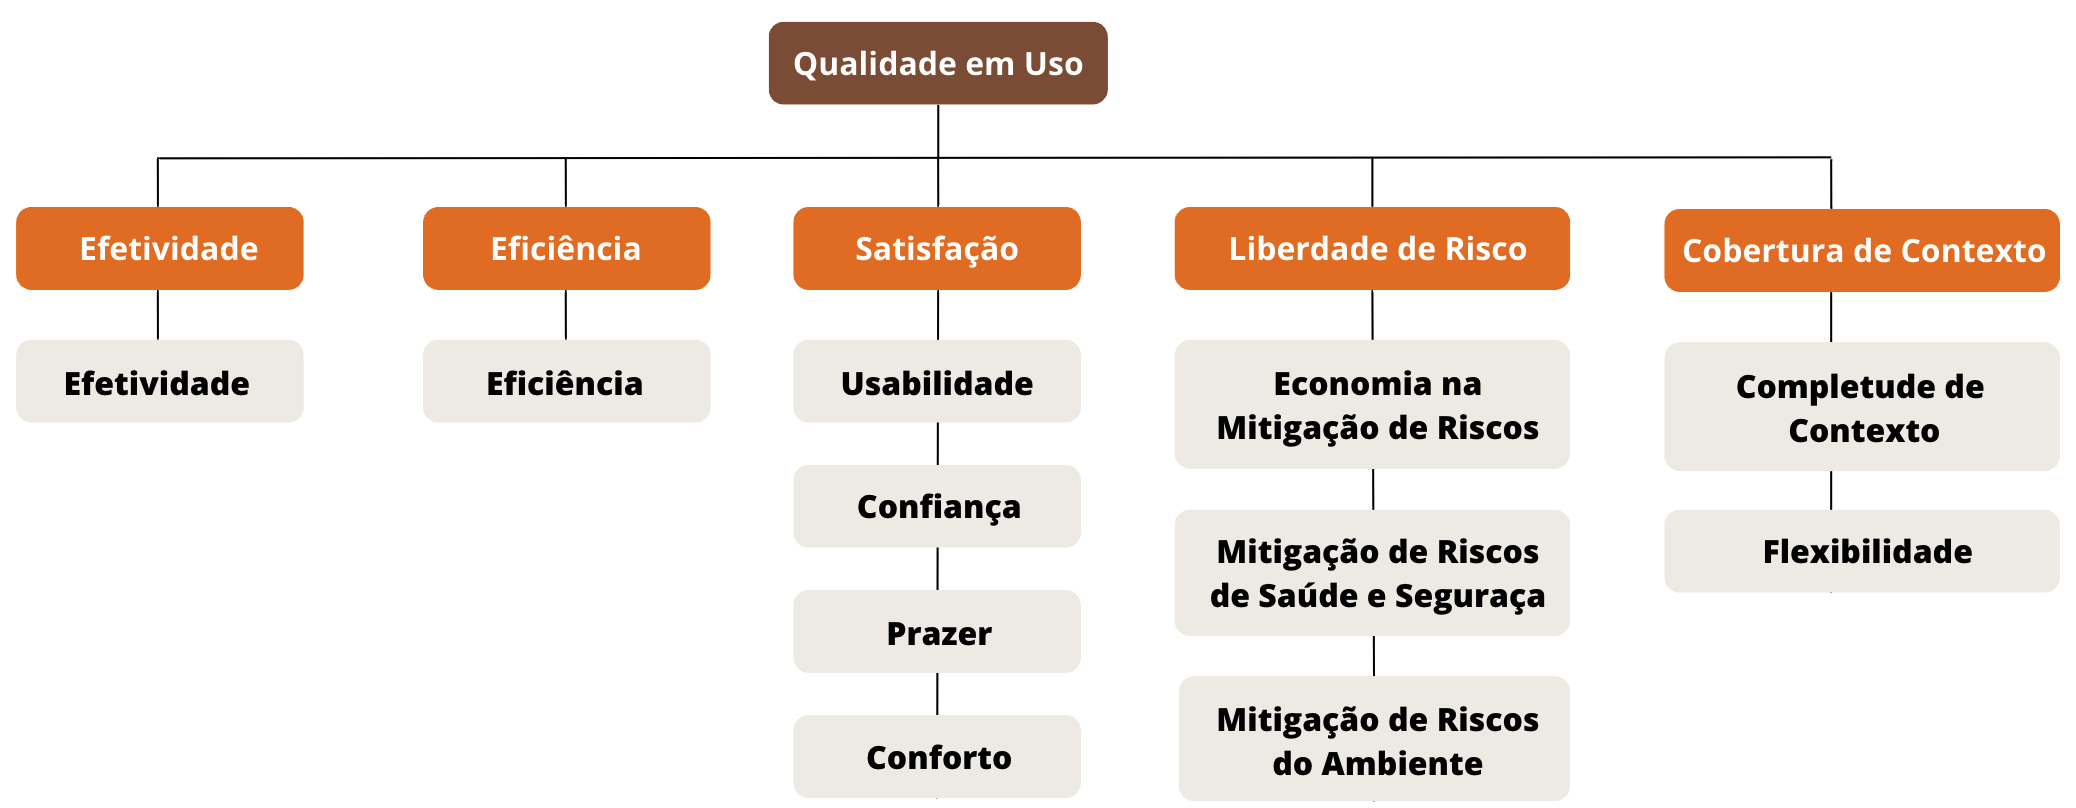
\includegraphics[width=1\linewidth]{figuras/quality_in_use.png}
% \text Fonte: Adaptado da Norma \citeonline{iso25010}
% \label{fig:model-quality-in-use}
% \end{figure}

\section{Problema}

Mesmo com o conhecimento de especialistas de negócio e de gerentes de produto, prever as necessidades do usuário é, na maioria das vezes, impreciso \cite{castellion2008do}. Além disso, a coleta direta de opiniões dos usuários também pode não ser assertiva, já que, aquilo que um usuário imagina que deseja muitas vezes difere do que ele realmente utilizaria na prática. Além disso, generalizar os resultados de uma análise qualitativa nem sempre é viável ou ideal \cite{cao2008agile}.

Considerando essa conjuntura, a análise quantitativa por meio de experimentos se apresenta como uma alternativa mais precisa, com a formalização de hipóteses e a definição de métricas-chave para observação \cite{kohavi_oce_and_ab_tests_2017}. No entanto, esse processo exige uma instrumentação adequada para garantir a confiabilidade estatística dos testes realizados. Para isso, é essencial uma definição sistemática do processo de desenvolvimento, incluindo a coleta e análise de dados.

A literatura apresenta diferentes modelos e técnicas para o desenvolvimento orientado a dados, porém carece de uma compreensão compartilhada sobre definições, processos e estratégias, o que dificulta a adoção da prática \cite{quin_b_2024}. Assim, \textbf{a falta de sistematização da coleta e da análise de dados torna a avaliação da qualidade em uso de um produto mais difícil e, muitas vezes, imprecisa}. Esse cenário faz com que a priorização do que será desenvolvido se baseie apenas em opiniões dos envolvidos na construção do produto, ao invés de um processo orientado à tomada de decisão baseada em dados \cite{olsson_opinions_2014}.

\section{Questão de Pesquisa} 
\label{sec:questao}

Para definir a questão de pesquisa norteadora deste trabalho foi utilizada a abordagem \textit{Goal Question Metric} (GQM), que propõe a especificação hierárquica de objetivos, questões e métricas de maneira \textit{top-down}, vide Figura \ref{fig:GOAL_QUESTION_METRIC}. O propósito desta abordagem é tornar o planejamento e a mensuração dos objetivos de uma pesquisa em questões e métricas que embasem suas respostas. Seguindo essa estrutura e a adaptando para o contexto desta pesquisa, definiram-se as seguintes características: propósito, foco, objeto de estudo e ponto de vista (vide Tabela \ref{tab:gqm}). Com isso, foi formulada a questão de pesquisa norteadora deste trabalho:

\begin{figure}[h] 
    \centering
    \caption{Estrutura do Modelo GQM}
    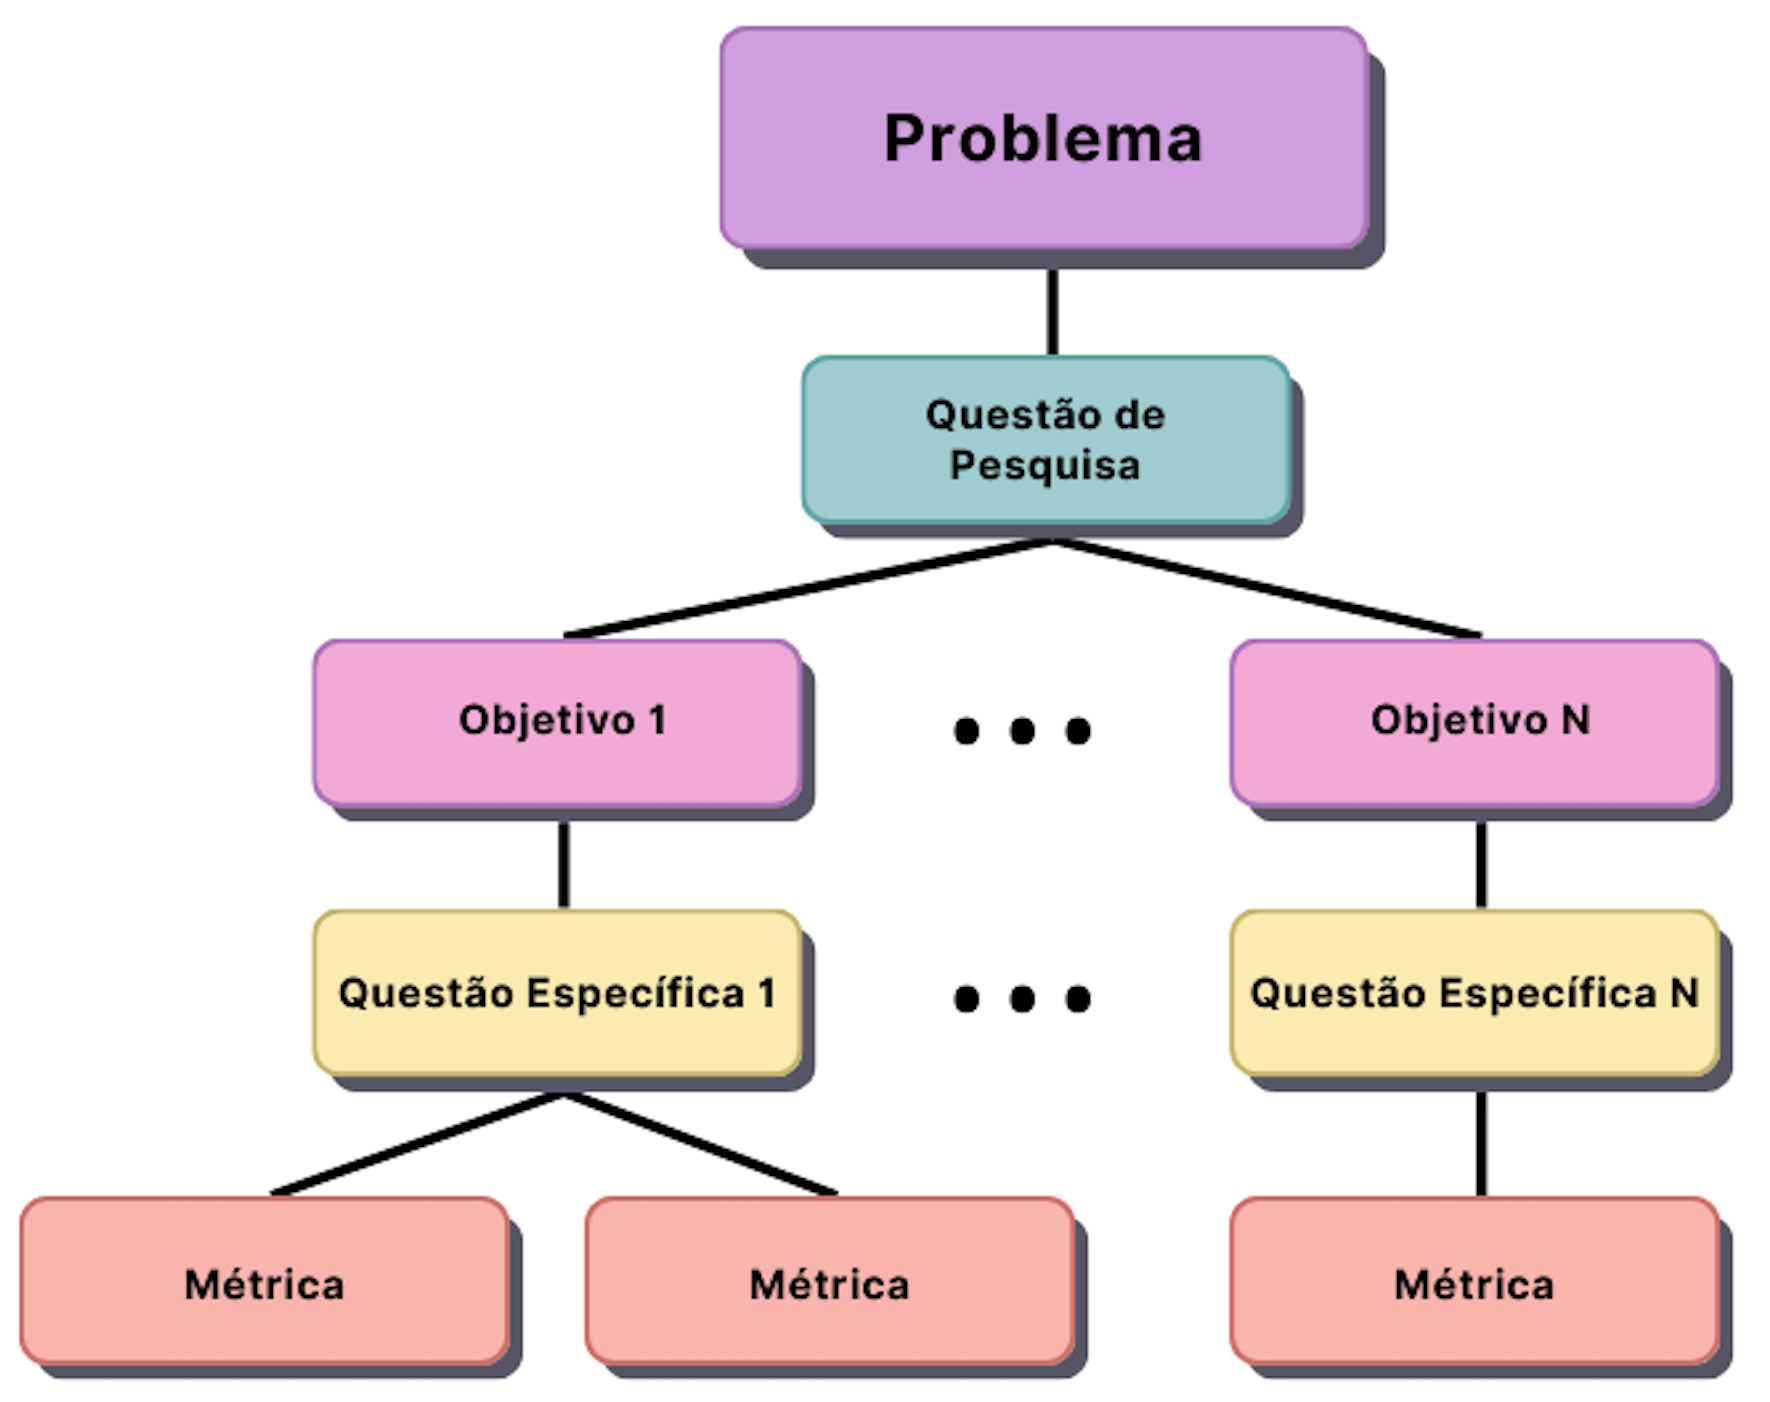
\includegraphics[width=0.75\textwidth]{figuras/gqm.png}

    \begin{center}
    \text Fonte: Adaptado de  \citeonline{basili_goal_1994}
    
    \end{center}
    \label{fig:GOAL_QUESTION_METRIC}
\end{figure}


\begin{table}[h!]
\centering
    \caption{Características de Definição da Questão de Pesquisa}
        \begin{tabular}{|p{4cm}|p{10cm}|}
            \hline
            \textbf{Característica} & \textbf{Valor} \\
            \hline
            Analisar & Versões de produto de \textit{software} \\
            Propósito & Avaliar \\
            Foco & Adoção de práticas de experimentação contínua para embasar a tomada de decisão na implantação de novas versões de um produto de \textit{software} \\
            Objeto de Estudo & Produto de \textit{Software} \\
            Ponto de Vista & Pesquisador \\
            Contexto & Manutenção e evolução de um produto de \textit{software}, em uma organização privada brasileira \\
            \hline
        \end{tabular}
   
 
    \begin{center}
        \text{Fonte: Adaptado de \citeonline{basili_goal_1994}}   
    \end{center}

    \label{tab:gqm}
\end{table}



\begin{center}
    \textit{Como a adoção de práticas de experimentação contínua pode auxiliar a tomada de decisão sobre a implantação de novas versões de um produto de software?}   
\end{center}



\section{Objetivos}
\label{subsec:objetivos-pesquisa}

O principal objetivo deste estudo é investigar como a adoção de práticas de experimentação contínua pode auxiliar na análise da qualidade em uso em um produto de \textit{software} e na tomada de decisão estratégica. Para alcançar esse objetivo geral, foram definidos os seguintes objetivos específicos, que deverão guiar a realização da primeira etapa deste trabalho:

\begin{itemize} 
    \item Realizar um levantamento teórico nas áreas de experimentação, qualidade de \textit{software}, análise estatística  de dados e desenvolvimento orientado a dados; 
    \item Adaptar o processo de desenvolvimento já existente no produto avaliado, incluindo práticas de experimentação contínua para posterior execução e avaliação; 
    \item Planejar um estudo de caso para observar a aplicação do processo proposto no ambiente real de desenvolvimento e uso do produto, objeto desta investigação;
    \item Executar as atividades propostas, coletar métricas de uso e comparar diferentes versões do produto de \textit{software}, avaliando estatisticamente qual delas foi melhor recebida pelos usuários. Ou seja, qual versão apresenta melhor atributo de qualidade em uso percebido. Além disso, documentar e analisar os resultados dos experimentos;
    \item Realizar uma coleta de opinião dos envolvidos no processo em relação às atividades realizadas; e 
    \item Analisar e documentar os principais achados deste estudo. 
\end{itemize}

% \section{Metodologia}

% \subsection{Classificação Metodológica}


% \begin{figure}[H]
% \centering
% \caption{Titulo da imagem}
% \includegraphics[width=1\textwidth]{figuras/secao-metodologia/Metodologia.png}
% \legend {Colocar aqui a legenda da figura}
% \label{fig:metodologia}
% \end{figure}

% \subsection{Plano Metodológico}
% Conforme Brereton et al (BRERETON et al., 2008), o processo de um estudo de
% caso possui quatro fases principais: Planejamento; Coleta de Dados; Análise de Dados; e
% Relatórios, que compõem o plano metodológico adotado neste trabalho:

% O plano metodológico é baseado em \citeonline{brereton_2008}, que apresenta um \textit{Protocolo de Estudo de Caso}, com vários itens a serem desenvolvidos, e esses distribuídos em quatro grandes fases: Planejamento; Coleta de Dados; Análise de Dados; e Relatórios.

% Essas fases compreendem, de forma resumida:

% \begin{itemize}
%     \item \textbf{Planejamento da Pesquisa:} nessa fase apresenta-se o contexto do pesquisa com a revisão bibliográfica, pergunta de pesquisa,  definição dos objetivos do trabalho e a definição de um plano metodológico, com as escolhas metodológicas;
    
%     \item \textbf{Coleta dos Dados:} essa fase compreende o levantamento e a aplicação das técnicas de coleta de dados como revisão documental, revisão bibliográfica e estudo de caso;
    
%     \item \textbf{Análise dos Dados:} nessa fase realizam-se a interpretação e análise dos dados coletados, assim como a análise da validade do trabalho, cuja meta é avaliar a percepção dos gestores da empresa em relação as diretrizes propostas;
    
%     \item \textbf{Relatório:} por fim, o relatório é constituído pelos resultados deste trabalho e caracterizado por esta monografia.
% \end{itemize}

% O planejamento metodológico do \textit{Protocolo de Estudo de Caso} \cite{brereton_2008} é apresentado no Capítulo Proposta (REVISAR - ALINHAR COM NOVA ESTRUTURA).



\section{Organização do Trabalho}
\label{sec:organizacao}

Esta subseção visa apresentar a estrutura do documento e o que está presente em cada capítulo desta monografia.

\begin{itemize}
    \item \textbf{Introdução:} apresentação do trabalho, do seu contexto e problemática, além da sua questão de pesquisa e objetivos;
    \item \textbf{Referencial Teórico:} fundamentação teórica do presente trabalho; explanação sobre os principais tópicos relacionados ao contexto desta pesquisa: experimentação em \textit{software}, qualidade de \textit{software}, experimentos controlados, análise de dados e experimentação contínua;
    \item \textbf{Revisão Estruturada da Literatura:} metodologia empregada para a seleção dos estudos que compõem o material bibliográfico; descrição do protocolo utilizado para busca e seleção dos artigos, bem como os resultados desta pesquisa;
    \item \textbf{Proposta de Estudo de Caso:} descrição da estratégia de pesquisa e seu protocolo; definição dos objetivos e da questão de pesquisa; definição e apresentação das atividades a serem realizadas na segunda parte desta monografia; e
    \item \textbf{Condições do Trabalho:} visão geral sobre a situação atual desta investigação; apresentação das atividades já concluídas e daquelas que serão realizadas na segunda etapa desta monografia.
\end{itemize}


\section{Cronograma e Fluxo de Atividades}\label{cronograma}

\subsection{Atividades da Primeira Etapa}
\label{cronograma1}

Esta subseção visa discriminar as atividades realizadas na primeira etapa do trabalho, os apresentando também em forma de fluxo na Figura \ref{fig:atividades_1} e às dispondo cronologicamente na Figura \ref{fig:cronograma_1}.

\begin{itemize}
    \item \textbf{Contextualização em Experimentação na Engenharia de Software:} leituras com o intuito de compreender o processo de experimentação e a abordagem científica necessária para a realização da Revisão da Literatura da primeira parte desta pesquisa, bem como do Estudo de Caso e do Experimento que serão realizados na segunda parte;
    \item \textbf{Contextualização em Experimentação Contínua:} leitura de materiais referentes ao processo de Experimentação Contínua e Desenvolvimento Orientado a Dados com o objetivo de compreender o estado da arte, identificar as lacunas existentes e moldar os objetivos deste trabalho; consumo de materiais para capacitação do pesquisador nas áreas de qualidade de software e experimentos científicos;
    \item \textbf{Definição dos Objetivos e Protocolo de Pesquisa:} definição do protocolo de revisão da literatura e dos objetivos da pesquisa segundo a abordagem GQM \cite{basili_goal_1994}, além dos objetivos específicos e da questão de pesquisa do trabalho; formulação do protocolo de pesquisa conforme proposto por \citeonline{kitchenham_rsl}: questões de pesquisa da revisão, \textit{string} de busca, critérios de inclusão e exclusão e formulário de extração de dados;
    \item \textbf{Busca e Seleção dos Artigos:} execução da \textit{string} de busca e seleção do primeiro grupo de artigos a partir da leitura de título e resumo; processo de \textit{snowballing} a partir dos artigos selecionados, selecionando novos materiais a partir da leitura parcial dos mesmos (título e resumo e, caso necessário, introdução e conclusão);
    \item \textbf{Leitura do Material Selecionado:} leitura integral do material selecionado com o objetivo de compreender o estado da arte, conhecer os modelos e processos já existentes e construir o corpo de conhecimento necessário para a formulação da proposta de estudo de caso;
    \item \textbf{Definição da Proposta de Processo:} elaboração da proposta de processo de experimentação; formalização da proposta de estudo de caso, discriminando objetivos, objeto, instrumentalização e atividades a serem realizadas;
    \item \textbf{Escrita do Trabalho:} redação da monografia seguindo a organização apresentada na Seção \ref{sec:organizacao};
    \item \textbf{Revisão da Monografia:} revisão e correção; e
    \item \textbf{Apresentação do Trabalho:} apresentação da primeira parte desta monografia para a banca avaliadora.
\end{itemize}

\begin{figure}
    \caption{Fluxo de Atividades Realizadas na Primeira Etapa Desta Monografia}
    \centering
    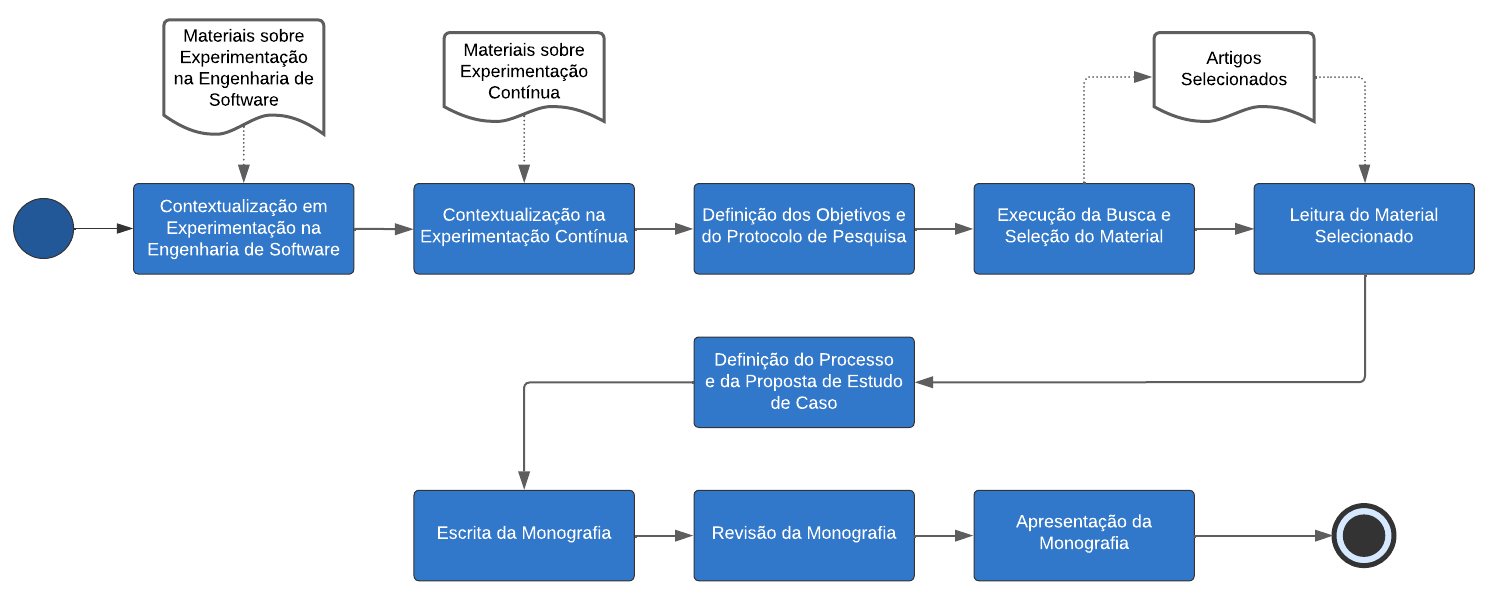
\includegraphics[width=1\linewidth]{figuras/atividades1.png}
    \text{Fonte: Autor}
    \label{fig:atividades_1}
\end{figure}

\begin{figure}
    \caption{Cronograma Realizado na Primeira Etapa da Monografia}
    \centering
    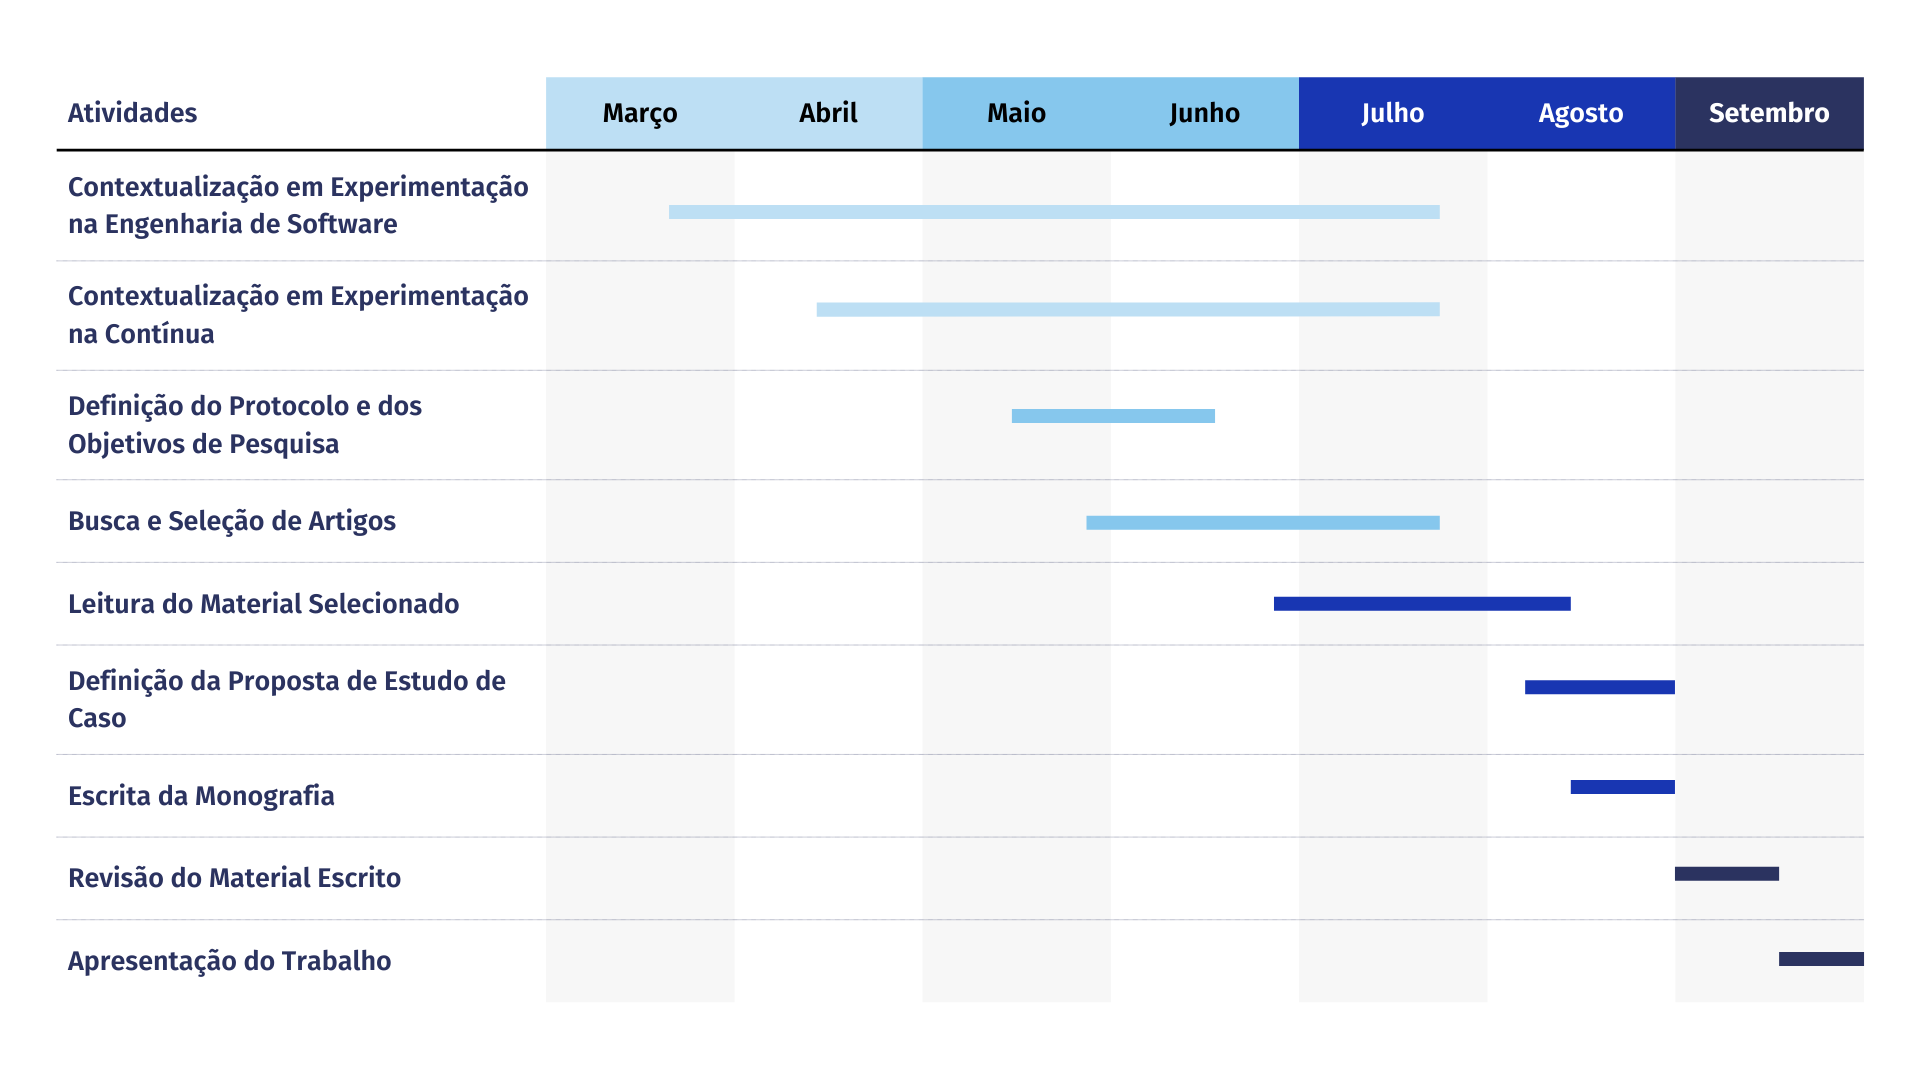
\includegraphics[width=1\linewidth]{figuras/cronograma1.png}
    \text{Fonte: Autor}
    \label{fig:cronograma_1}
\end{figure}


\subsection{Atividades da Segunda Etapa}
\label{cronograma2}

Esta subseção visa apresentar as atividades planejadas para a segunda etapa deste trabalho,
as apresentando em forma de fluxo na Figura \ref{fig:atividades_2} e as dispondo em forma de cronograma na Figura \ref{fig:cronograma_2}.

\begin{itemize}
    \item \textbf{Evolução do Trabalho:} revisão e atualização do material já escrito a partir das considerações da banca avaliadora;
    \item \textbf{Formulação de Hipóteses:} realização das atividades referentes à Engenharia de Hipóteses; geração, documentação e priorização de hipóteses para escolher aquela que será desenvolvida e observada através da execução do experimento objeto do Estudo de Caso deste trabalho;
    \item \textbf{Instrumentação do Experimento:} prototipação da hipótese selecionada; definição das métricas escolhidas para validação da hipótese; preparo dos disparos de evento para coleta dos dados; validação do \textit{design do experimento}; revisão da hipótese ou das métricas elencadas, caso necessário;
    \item \textbf{Desenvolvimento e Coleta de Dados:} desenvolvimento da nova versão de software (tratamento) a ser comparada com a versão já existente (controle); liberação da nova versão para os usuários beta a fim de iniciar a iteração do experimento (a coleta de dados já deve acontecer a partir desta liberação);
    \item \textbf{Análise de Dados:} iteração no experimento caso necessário (como, por exemplo, dados coletados insuficientes, necessidade de prolongamento do experimento); análise dos dados coletados para os testes de hipótese; decisão sobre a liberação da versão de tratamento para todos os usuários ou abandono da mesma;
    \item \textbf{Documentação do Resultado do Experimento:} documentação dos resultados do teste da hipótese para registro e criação de um corpo de conhecimento que auxilie futuros experimentos;
    \item \textbf{Coleta de Percepção dos Envolvidos:} pesquisa de opinião com os colaboradores envolvidos no estudo de caso para avaliação do processo proposto;
    \item \textbf{Análise dos Resultados do Estudo de Caso:} resposta às questões de pesquisa do estudo de caso a partir dos dados coletados, com posterior resposta à principal questão de pesquisa; descrição do processo realizado e documentação dos resultados obtidos;
    \item \textbf{Revisão da Monografia:} revisão e correção minuciosa do trabalho em busca de possíveis correções ou atualizações necessárias, tanto por parte do pesquisador quanto do orientador; e
    \item \textbf{Apresentação do Trabalho Finalizado:} apresentação da monografia finalizada à banca avaliadora.
\end{itemize}

\begin{figure}
    \caption{Fluxo de Atividades Planejadas Para a Segunda Etapa da Monografia}
    \centering
    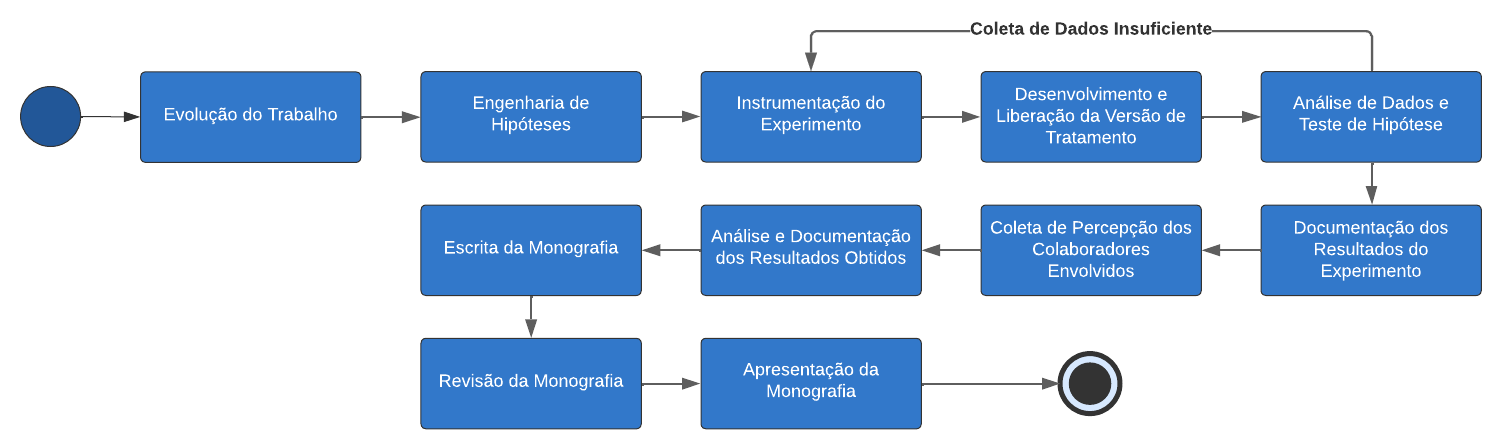
\includegraphics[width=1\linewidth]{figuras/atividades2.png}
    \text{Fonte: Autor}
    \label{fig:atividades_2}
\end{figure}
\begin{figure}
    \caption{Cronograma Planejado Para a Segunda Etapa da Monografia}
    \centering
    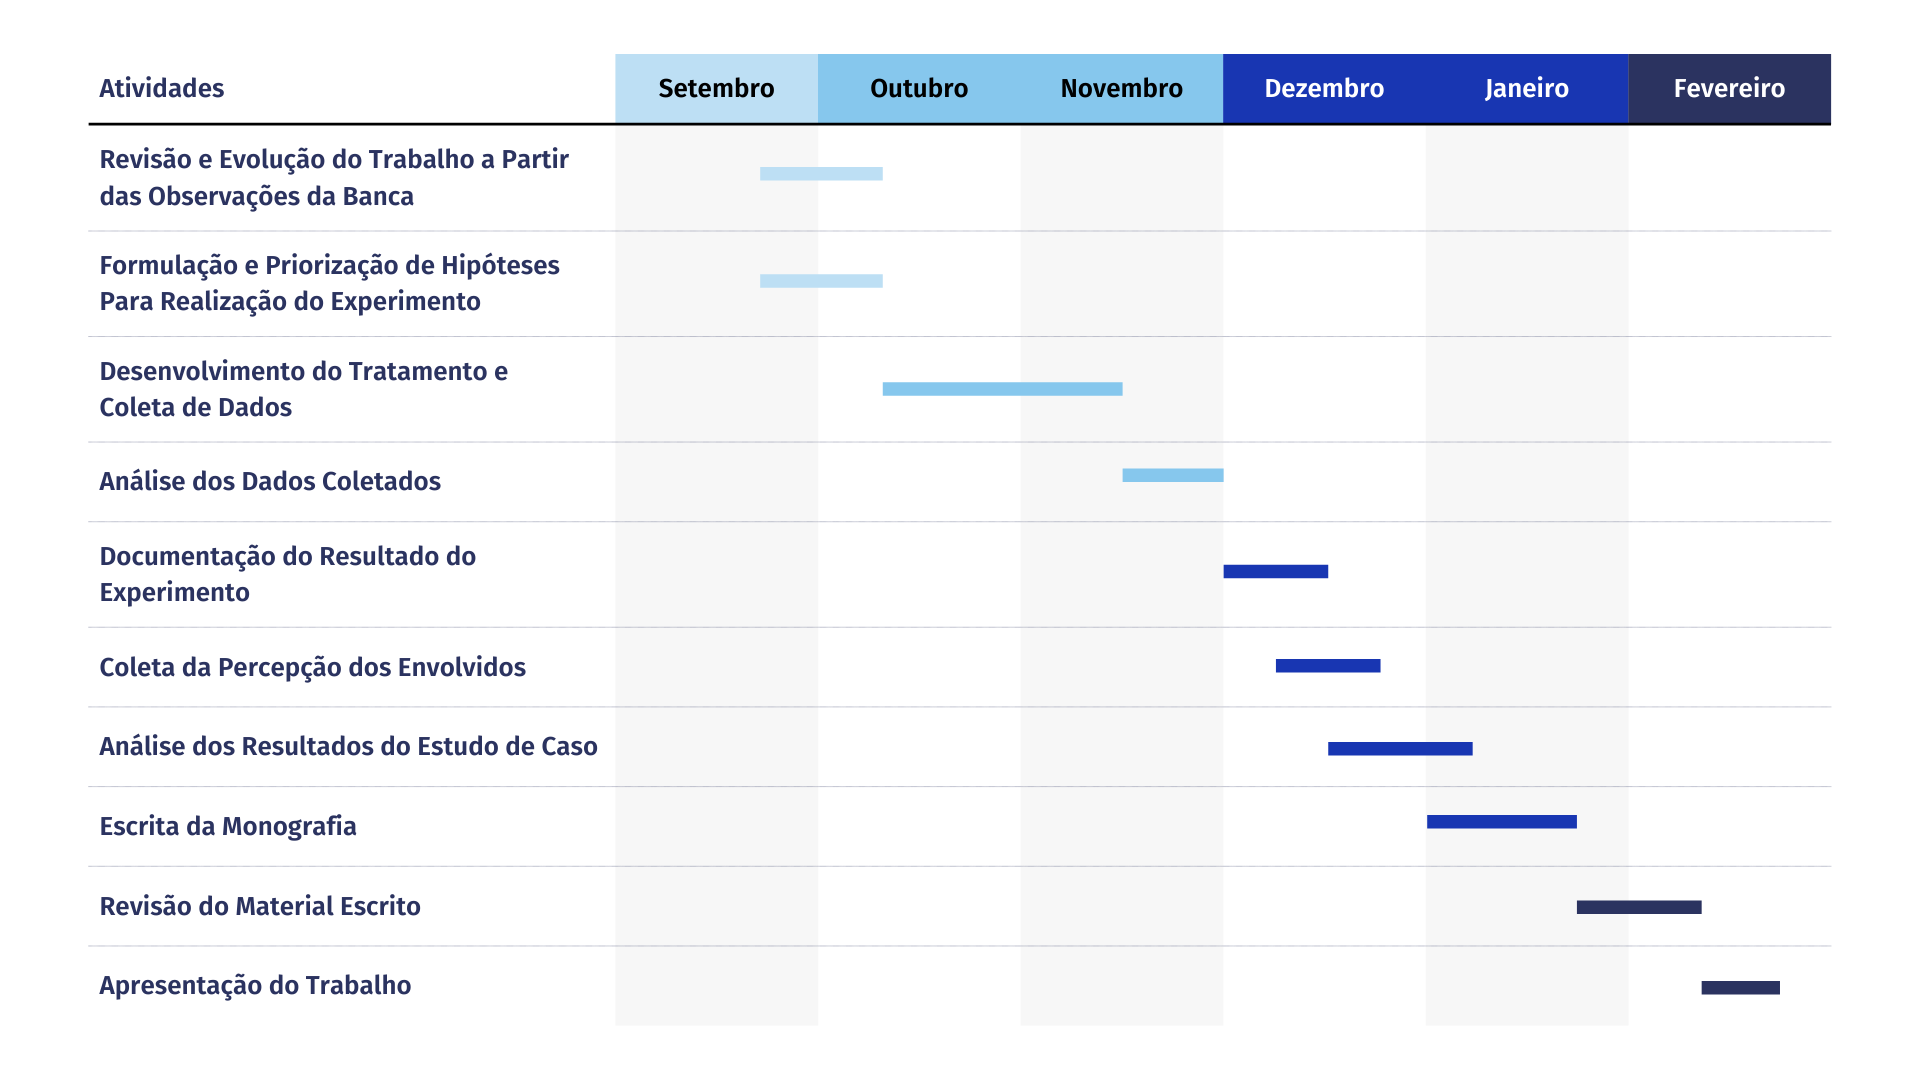
\includegraphics[width=1\linewidth]{figuras/cronograma2.png}
    \text{Fonte: Autor}
    \label{fig:cronograma_2}
\end{figure}
